\chapter{Méthodes variationnelles} \label{chap:Ch09}
\section{Théoremes variationnels} \label{sec:Ch09-1}
Dans tout ce chapitre, nous nous intéresserons à un problème statique régulier (paragraphe~\ref{ssec:Ch07-1.1}) pour un matériau élastique linéaire quelconque (isotrope ou anisotrope) caractérisé par un tenseur d'élasticité $A_{ijkh}$.
Pour simplifier l'écriture, nous supposerons le matériau homogène, $A_{ijkh} =$ Cte et nous prendrons les CL sous la forme mixte \eqref{eq:Ch07-007}.
Pour un autre problème régulier, l'écriture serait plus lourde, mais les résultats et les raisonnements seraient identiques.

\subsection{Notions fondamentales} \label{ssec:Ch09-1.1}
Nous cherchons donc un champ de déplacements et un champ de contraintes vérifiant les équations suivantes
\begin{align}
    & \sigma_{ij,j} + f_i = 0 \label{eq:Ch09-001} \\
    & \sigma_{ij} n_j |_{S_f} = T_i^d \label{eq:Ch09-002} \\
    & u_i |_{S_u} = u_i^d \label{eq:Ch09-003} \\
    & \sigma_{ij} = A_{ijkh} \varepsilon_{kh} \label{eq:Ch09-004} \\
    & \varepsilon_{ij} = \frac{1}{2} \left( u_{i,j} + u_{j,i} \right) \label{eq:Ch09-005}
\end{align}

Parmi ces équations, certaines sont de nature statique et portent uniquement sur les contraintes -- les équations~\eqref{eq:Ch09-001} et \eqref{eq:Ch09-002} -- d'autres sont de  nature cinématique  et portent uniquement  sur  les déplacements -- \eqref{eq:Ch09-003}.  
Enfin, un troisième groupe d'équations -- \eqref{eq:Ch09-004} -- relie les contraintes et les déplacements.

\begin{deff}
    Un champ de déplacements $\tilde{u}_i$ est un champ cinématiquement admissible ($\tilde{u}_i$ est un CCA) s'il vérifie les conditions cinématiques \eqref{eq:Ch09-003}.
    \begin{equation}
        u_i |_{S_u} = u_i^d
        \label{eq:Ch09-006}
    \end{equation}
\end{deff}

Partant d'un CCA $\tilde{u}_i$, on peut lui associer un champ de déformations $\tilde{\varepsilon}_{ij}$ par \eqref{eq:Ch09-005}, puis un champ de contraintes $\tilde{\sigma}_{ij}$ par la loi de comportement \eqref{eq:Ch09-004}, mais ce champ de contraintes n'a aucune raison de vérifier les conditions statiques \eqref{eq:Ch09-001} et \eqref{eq:Ch09-002}. 

\begin{deff}
    Un champ de contraintes $\hat{\sigma}_{ij}$ est un champ statiquement admissible ($\hat{\sigma}_{ij}$ est un CSA) s'il vérifie les conditions statiques \eqref{eq:Ch09-001} et \eqref{eq:Ch09-002}
    \begin{equation}
        \sigma_{ij,j} + f_i = 0 \quad,\quad \sigma_{ij} n_j |_{S_f} = T_i^d
        \label{eq:Ch09-007}
    \end{equation}
\end{deff}

Partant d'un CSA $\hat{\sigma}_{ij}$ on peut lui associer un champ de déformations $\varepsilon$ par la loi de comportement \eqref{eq:Ch09-004}, mais, puisque $\hat{\sigma}_{ij}$ ne doit pas vérifier les équations de Beltrami, on ne pourra en général pas calculer un $\hat{u}_i$ par intégration de \eqref{eq:Ch09-005}.
\textit{A fortiori}, les conditions \eqref{eq:Ch09-003} ne seront elles pas vérifiées.

Avec cette terminologie, le problème d'élasticité \eqref{eq:Ch09-001} à \eqref{eq:Ch09-005} se ramène à la recherche d'un CCA $\hat{u}_i$ et d'un CSA $\hat{\sigma}_{ij}$ reliés par la loi de comportement \eqref{eq:Ch09-004}.
Toute la suite de ce chapitre sera basée sur le lemme suivant -- généralisation du théorème des travaux virtuels \eqref{eq:Ch03-046}.

\newtheorem*{lfond}{Lemme fondamental}
\begin{lfond}
    Soit ${\mathop{u}^{\ast}}_i$ un champ de déplacements (virtuels) quelconque et $\hat{\sigma}_{ij}$ un CSA, alors
    \begin{equation}
        \iiint_{\Omega} \hat{\sigma}_{ij} {\mathop{\varepsilon}^{\ast}}_{ij} \ud v = \iiint_{\Omega} f_{i} {\mathop{u}^{\ast}}_i \ud v + \iint_{\partial \Omega} \hat{\sigma}_{ij} n_j {\mathop{u}^{\ast}}_i \ud S
        \label{eq:Ch09-008}
    \end{equation}
\end{lfond}
\begin{proof}
    La  démonstration  est directement calquée sur celle du paragraphe~\ref{ssec:Ch01-2.1}.
    Nous partons du premier membre et utilisons la symétrie de $\hat{\sigma}_{ij}$.
    \begin{align*}
        \iiint_{\Omega} \hat{\sigma}_{ij} {\mathop{\varepsilon}^{\ast}}_{ij} \ud v &= \frac{1}{2} \iiint_{\Omega} \hat{\sigma}_{ij} \left( {\mathop{u}^{\ast}}_{i,j} + {\mathop{u}^{\ast}}_{j,i}  \right) \ud v = \iint_{\Omega} \hat{\sigma}_{ij} {\mathop{u}^{\ast}}_{i,j} \ud v \\
        & = \iiint_{\Omega} \left( \hat{\sigma}_{ij} {\mathop{u}^{\ast}}_{i} \right)_{,j} \ud v - \iiint_{\Omega} \hat{\sigma}_{ij,j}  {\mathop{u}^{\ast}}_{i} \ud v
    \end{align*}
    Par utilisation du théorème de la divergence, le premier terme donne l'intégrale de surface du second membre de \eqref{eq:Ch09-008}, tandis que le second terme donne l'intégrale de volume par \eqref{eq:Ch09-007}.
    On retrouve le théorème des travaux virtuels en prenant comme CSA $\hat{\sigma}_{ij}$ le champ solution $\sigma_{ij}$.
\end{proof}

\newtheorem*{ttv}{Théorème des travaux virtuels}
\begin{ttv}
    Pour tout champ de déplacements virtuels ${\mathop{u}^{\ast}}_{i}$
    \begin{equation}
        \iiint_{\Omega} \sigma_{ij} {\mathop{\varepsilon}^{\ast}}_{ij} \ud v = \iiint_{\Omega} f_i {\mathop{u}^{\ast}}_i \ud v + \iint_{\partial \Omega} \sigma_{ij} n_j {\mathop{u}^{\ast}}_i \ud S
        \label{eq:Ch09-009}
    \end{equation}
\end{ttv}

D'un point de vue algébrique, et en revenant à la structure décrite à la fin du paragraphe~\ref{ssec:Ch03-2.3}, on peut généraliser \eqref{eq:Ch03-050} en
\begin{equation}
    \langle \langle \mathop{\varepsilon}^{\ast}, \hat{\sigma} \rangle \rangle = \langle \mathop{u}^{\ast}, \varphi \rangle
    \label{eq:Ch09-010}
\end{equation}
valable pour tout champ de déplacements ${\mathop{u}^{\ast}}_i$ et tout CSA $\hat{\sigma}_{ij}$.
Plus précisément, on a la situation suivante
\[
\begin{CD}
    \mathcal{C} @>{\text{dualité } \langle\ ,\ \rangle}>> \mathcal{U} \\
    @AEAA    @VVDV \\
    \mathcal{S} @<<{\text{dualité } \langle\langle\ ,\ \rangle\rangle}< \mathcal{D}
\end{CD}
\]
L'opérateur $D$ est l'opérateur
\begin{equation}
    {\mathop{u}^{\ast}}_i \mapsto {\mathop{\varepsilon}^{\ast}}_{ij} = \frac{1}{2} \left(  \right)
    \label{eq:Ch09-011}
\end{equation}
donnant les déformations en fonction des déplacements, et l'opérateur $E$ est l'opérateur
\begin{equation}
    \hat{\sigma}_{ij} \mapsto \left( \hat{f}_i = - \hat{\sigma}_{ij,j}\ , \ \hat{T}_i = \hat{\sigma}_{ij} n_j \right)
    \label{eq:Ch09-012}
\end{equation}
associant au champ de contraintes $\hat{\sigma}_{ij}$ les forces volumiques $\hat{f}_i$ et les efforts de surface $\hat{T}_i$ qui lui correspondent.
La relation \eqref{eq:Ch09-010} montre que les opérateurs $D$ et $E$ sont adjoints l'un de l'autre.
C'est une structure que l'on retrouvera dans toutes les théories de Mécanique des Solides en petite perturbations.

Il faut remarquer que, bien que nous les ayons présentés dans un contexte d'élasticité, toutes les définitions et tous les résultats de ce paragraphe sont indépendants de la loi de comportement; en particulier, on les retrouvera en plasticité.
La loi de comportement se présente comme une relation entre les déformations et les contraintes (voir paragraphe~\ref{ssec:Ch04-1.3}).
En élasticité, cette relation est une application linéaire reliant les valeurs instantanées des déformations et des contraintes, cette application étant de plus supposée symétrique (auto-adjointe) et définie positive (paragraphe~\ref{ssec:Ch05-1.1}). 

\subsection{Le théorème de l'énergie potentielle} \label{ssec:Ch09-1.2}
Soit $\tilde{u}_i$ un CCA, on calcule $\tilde{\varepsilon}_{ij}$ par \eqref{eq:Ch09-005}, et on peut donc définir l'énergie de déformation du CCA $\tilde{u}_i$ par
\begin{equation}
    W(\tilde{\varepsilon}_{ij}) = \frac{1}{2} \iiint_{\Omega} A_{ijkh} \tilde{\varepsilon}_{ij} \tilde{\varepsilon}_{kh} \ud v = \frac{1}{2} \iiint_{\Omega} \tilde{\sigma}_{ij} \tilde{\varepsilon}_{ij} \ud v
    \label{eq:Ch09-013}
\end{equation}
On introduit également le travail des efforts (volumiques et surfaciques) donnés dans le deplacement $\tilde{u}_i$
\begin{equation}
    \tilde{T}_{f}^d (\tilde{u}_i) = \iiint_{\Omega} f_i \tilde{u}_i \ud v T_f^d (\tilde{u}_i) \quad,\quad T_f^d(\tilde{u}_i) = \iint_{S_f} T_i^d \tilde{u}_i \ud S
    \label{eq:Ch09-014}
\end{equation}
Pour les CL mixtes \eqref{eq:Ch06-007} choisies, le travail des efforts surfaciques donnés, $T_f^d$ s'exprime simplement.
Pour un problème régulier quelconque, l'expression peut être plus compliquée, mais, comme on l'a vu au paragraphe~\ref{ssec:Ch06-1.1}, le travail des efforts de surface se décompose sans ambiguïté en $T_u^d$ et $T_f^d$ (voir par exemple \eqref{eq:Ch06-010} et le paragraphe~\ref{ssec:Ch09-1.4}). 
\begin{defn}
    L'énergie potentielle du CCA $\tilde{u}_i$ est
    \begin{equation}
        K(\tilde{u}_i) = W(\tilde{\varepsilon}_{ij}) - \tilde{T}_f^d (\tilde{u}_i)
        \label{eq:Ch09-015}
    \end{equation}
\end{defn}
On 	démontre alors
\newtheorem*{ThEP}{Théorème de l'énergie potentielle}
\begin{ThEP}
    Parmi tous les CCA, la (ou les) solution $u_i$ minimise l'énergie potentielle
    \begin{equation}
        K(u_i) \leq K (\tilde{u}_i) \quad \forall \tilde{u}_i \text{ CCA}
        \label{eq:Ch09-016}
    \end{equation}
\end{ThEP}
\begin{proof}
    Soit $u_i$ une solution du problème \eqref{eq:Ch09-001} à \eqref{eq:Ch09-005}, et $\tilde{u}_i$ un CCA.
    Nous définissons
    \begin{equation}
        \tilde{u}_i = u_i + \tilde{u}_i^0 \quad,\quad \tilde{u}_i^0|_{S_u} = 0
        \label{eq:Ch09-017}
    \end{equation}
    et $u_i$ est un CCA pour le problème homogène associé 
    \begin{align*}
        K\left(\tilde{u}_i\right) &=\frac{1}{2} \iiint_{\Omega} A_{ijkh} \left( \varepsilon_{ij} + \tilde{\varepsilon}_{ij}^0 \right) \left( \varepsilon_{kh} + \tilde{\varepsilon}_{kh}^0 \right) \ud v - \iiint_{\Omega} f_i \left( u_i + \tilde{u}_i^0 \right) \ud v - \iint_{S_f} T_i^d \left( u_i + \tilde{u}_i^0 \right) \ud S \\
        &= K\left( u_i \right) + \frac{1}{2} \iiint_{\Omega} A_{ijkh} \tilde{\varepsilon}_{ij}^0 \tilde{\varepsilon}_{kh}^0 \ud v + \iiint_{\Omega} A_{ijkh} \tilde{\varepsilon}_{ij}^0 \varepsilon_{kh} \ud v - \iiint_{\Omega} f_i \tilde{u}_i^0 \ud v - \iint_{S_f} T_i^d \tilde{u}_i^0 \ud S
    \end{align*}
    Mais $u_i$ est solution, et le théorème des travaux virtuels \eqref{eq:Ch09-009} donne, en prenant ${\mathop{u}^{\ast}}_i = \tilde{u}_i^0$
    \begin{align*}
        \iiint_{\Omega} A_{ijkh} \tilde{\varepsilon}_{kh}^0 \ud v &= \iint_{\Omega} \sigma_{ij} \tilde{\varepsilon}_{ij}^0 \ud v \\
        &= \iiint_{\Omega} f_i \tilde{u}_i^0 \ud v + \iint_{\partial \Omega} \sigma_{ij} n_j \tilde{u}_i^0 \ud S \\
        &= \iiint_{\Omega} f_i \tilde{u}_i^0 \ud v + \iint_{S_f} T_i^d \tilde{u}_i^0 \ud S + \iint_{S_u} \cancel{\sigma_{ij} n_j \tilde{u}_i^0} \ud S
    \end{align*}
    puisque sur $S_f$, on a \eqref{eq:Ch09-002}, et que, d'après \eqref{eq:Ch09-003} et \eqref{eq:Ch09-006}, $\tilde{u}_i^0$ est nul sur $S_u$.
    Finalement, on obtient donc
    \begin{equation}
        K\left( \tilde{u}_i \right) = K \left( u_i \right) + \frac{1}{2} \iiint_{\Omega} A_{ijkh} \tilde{\varepsilon}_{ij}^0 \tilde{\varepsilon}_{kh}^0 \ud v
        \label{eq:Ch09-018}
    \end{equation}
    Or le second terme est positif, puisque la matrice d'élasticité est définie positive (paragraphe~\ref{ssec:Ch05-1.1}).
    Ceci démontre \eqref{eq:Ch09-016}.
\end{proof}

On tire également de cette démonstration 
\newtheorem*{ThEU}{Théorème d'existence et d'unicité}
\begin{ThEU}
    Pour un problème de type I ou un problème mixte, il existe une solution unique.
    Pour un problème de type II. il existe une solution définie à un mouvement de solide rigide près si-et-seulement-si
    \begin{equation}
        \begin{split}
            \iiint_{\Omega} f_i \ud v + \iint_{\partial \Omega} T_i^d \ud S = 0 \\
            \iiint_{\Omega} \varepsilon_{ijk} x_{j} f_k \ud v + \iint_{\partial \Omega} \varepsilon_{ijk} x_j T_k^d = 0
        \end{split}
        \label{eq:Ch09-019}
    \end{equation}
    c'est à dire si-et-seulement-si les efforts appliqués forment un torseur nul. 
\end{ThEU}
\begin{proof}
    \textit{Unicité.}
    Soit $u_i^1$ et $u_i^2$ deux solutions, ils sont aussi CCA, et l'application de \eqref{eq:Ch09-016} montre que 
    \begin{displaymath}
        K\left( u_i^1 \right) = K \left( u_i^2 \right)
    \end{displaymath}
    soit, d'après \eqref{eq:Ch09-018}
    \begin{eqnarray}
        \iiint_{\Omega} A_{ijkh} \left( \varepsilon_{ij}^1 - \varepsilon_{ij}^2 \right) \left( \varepsilon_{kh}^1 - \varepsilon_{kh}^2 \right) \ud v = 0
        \label{eq:Ch09-020}
    \end{eqnarray}
    Il en résulte, puisque $A_{ijkh}$ est défini positif 
    \begin{equation}
        \varepsilon_{ij}^1 = \varepsilon_{ij}^2 \quad,\quad u_i^1 = u_i^2 + \varepsilon_{ijkh} \omega_j x_k + \alpha_i
        \label{eq:Ch09-021}
    \end{equation}
    et les deux solutions ne diffèrent que d'un mouvement de solide.
    Si $S_u$ existe (plus précisément, si $S_u$ est de mesure nulle), les CL en déplacements permettent de montrer que $\vec{\omega} = \vec{\alpha} = 0$ 
et donc $u_i^1 = u_i^2$ d'où l'unicité. 
    Par contre, si $S_u$ est vide (problème de type II), on ne peut plus éliminer ce mouvement de solide qui reste indéterminé.

    \textit{Existence.}
    L'existence d'une solution peut par exemple se démontrer en construisant, dans un espace fonctionnel approprié, une suite minimisante pour la fonctionnelle $K$ -- voir cours de Mathématiques.
    Pour un problème de type II, la condition d'équilibre \eqref{eq:Ch09-019} apparaît naturellement, car sinon la fonctionnelle n'est pas minorée. 
    Pour les autres problèmes, cette condition d'équilibre n'apparaît pas, car les efforts donnés sont équilibrés par les efforts de liaison (inconnus \textit{a priori}) s'exerçant à travers $S_u$.
\end{proof}

\subsection{Le théorème de l'énergie complémentaire} \label{ssec:Ch09-1.3}
Si nous partons d'un CSA $\hat{\sigma}_{ij}$, nous définissons son énergie de déformation par
\begin{equation}
    \hat{W}\left( \hat{\sigma}_{ij} \right) = \frac{1}{2} \iiint_{\Omega} \Lambda_{ijkh} \hat{\sigma}_{ij} \hat{\sigma}_{kh} \ud v = \frac{1}{2} \iiint_{\Omega} \hat{\sigma}_{ij} \hat{\varepsilon}_{ij} \ud v
    \label{eq:Ch09-022}
\end{equation}
et son travail dans les déplacements donnés par 
\begin{equation}
    T_{u}^d \left( \hat{\sigma}_{ij} \right) = \iint_{S_u} \hat{\sigma}_{ij} n_j u_i^d \ud S
    \label{eq:Ch09-023}
\end{equation}
et nous définissons 
\begin{defn}
    L'énergie complémentaire du CSA est
    \begin{equation}
        H \left( \hat{\sigma}_{ij} \right) = T_{u}^d \left( \hat{\sigma}_{ij} \right) - \hat{W}\left( \hat{\sigma}_{ij} \right)
        \label{eq:Ch09-024}
    \end{equation}
\end{defn}
et on obtient le résultat suivant 
\newtheorem*{ThECp}{Théorème de l'énergie complémentaire}
\begin{ThECp}
    Parmi tous les CSA, la solution $\sigma_{ij}$ maximise l'énergie complémentaire
    \begin{equation}
        H \left( \hat{\sigma}_{ij} \right) \leq H \left( \sigma_{ij} \right) \quad \forall \hat{\sigma}_{ij} \text{ CSA}
        \label{eq:Ch09-025}
    \end{equation}
\end{ThECp}
\begin{proof}
    Soit $\sigma_{ij}$ la solution, $\sigma_{ij}$ un CSA, et posons
    \begin{equation}
        \hat{\sigma}_{ij} = \sigma_{ij} + \hat{\sigma}_{ij}^0
        \label{eq:Ch09-026}
    \end{equation}
    et $\hat{\sigma}_{ij}^0$ est un CSA pour le problème homogène associé ($f_i^0 = 0,\ T_i^{d0} = 0$)
    \begin{equation}
        \hat{\sigma}_{ij,j}^0 = -f_i^0 = 0 \quad,\quad \hat{\sigma}_{ij}^0 n_j |_{S_f} = T_i^{d0} = 0
        \label{eq:Ch09-027}
    \end{equation}
    \begin{align*}
        H\left( \hat{\sigma}_{ij} \right) &= - \frac{1}{2} \iiint_{\Omega} \Lambda_{ijkh} \left( \sigma_{ij} + \hat{\sigma}_{ij}^0 \right) \left( \sigma_{kh} + \hat{\sigma}_{kh}^0 \right) \ud v + \iint_{S_u} \left( \sigma_{ij} + \hat{\sigma}_{ij}^0 \right) n_j u_i^d \ud S \\
        &= H\left( \sigma_{ij} \right) - \frac{1}{2} \iiint_{\Omega} \Lambda_{ijkh} \hat{\sigma}_{ij}^0 \hat{\sigma}_{kh}^0 \ud v - \iiint_{\Omega} \Lambda_{ijkh} \hat{\sigma}_{ij}^0 \sigma_{kh} \ud v + \iint_{S_u} \hat{\sigma}^0_{ij} n_j u_i^d \ud S
    \end{align*}
    En appliquant le lemme fondamental à $\hat{\sigma}_{ij}^0$ CSA pour le problème homogène associé, et à $u_i$, déplacement solution, on obtient
    \begin{align*}
        \iiint_{\Omega} \Lambda_{ijkh} \hat{\sigma}_{ij}^0 \sigma_{kh} \ud v &= \iiint_{\Omega} \hat{\sigma}_{ij}^0 \varepsilon_{ij} \ud v \\
        &= \cancel{\iint_{\Omega} f_i^0 u_i \ud v} + \cancel{\iint_{S_f} T_i^{d0} u_i \ud S} + \iint_{S_u} \hat{\sigma}_{ij}^0 n_j u_i \ud S
    \end{align*}
    Les deux premiers termes disparaissent d'après \eqref{eq:Ch09-027}, tandis que sur $S_u$, $u_i=u_i^d$ par \eqref{eq:Ch09-003}.
    Il vient finalement 
    \begin{equation}
        H \left( \hat{\sigma}_{ij} \right) = H \left( \sigma_{ij} \right) - \frac{1}{2} \iiint_{\Omega} \Lambda_{ijkh} \hat{\sigma}_{ij}^0 \hat{\sigma}_{kh}^0 \ud v
        \label{eq:Ch09-028}
    \end{equation}
    d'où la conclusion, puisque, comme $A_{ijkh}$, la matrice $\Lambda_{ijkh}$ est définie positive.
\end{proof}
\newtheorem*{ThComp}{Théorème de la comparaison}
\begin{ThComp}
    Soit $\left( u_i, \sigma_{ij} \right)$ la solution d'un problème régulier, $\tilde{u}_i$ un CCA et $\hat{\sigma}_{ij}$ un CSA
    \begin{equation}
        H \left( \hat{\sigma}_{ij} \right) \leq H \left( \sigma_{ij} \right) = K \left( u_i \right) \leq K \left( \tilde{u}_i \right)
        \label{eq:Ch09-029}
    \end{equation}
\end{ThComp}

Les deux théorèmes de l'énergie potentielle et de l'énergie complémentaire permettent d'écrire les deux inégalités.
Il reste donc à montrer l'égalité 
\begin{equation}
    K\left( u_i \right) = H\left( \sigma_{ij} \right)
    \label{eq:Ch09-030}
\end{equation}
pour la solution. 
\begin{proof}
    Pour la solution, on a 
    \begin{displaymath}
        W\left( u_i \right) = \hat{W} \left( \sigma_{ij} \right) = \frac{1}{2} \iiint_{\Omega} \sigma_{ij} \varepsilon_{ij} \ud v
    \end{displaymath}
    A partir de \eqref{eq:Ch09-015} et \eqref{eq:Ch09-024}, il vient alors
    \begin{displaymath}
        K\left( u_i \right) - H \left( \sigma_{ij} \right) = 2W - \tilde{T}_f^d \left( u_i \right) - T_u^d \left( \sigma_{ij} \right)
    \end{displaymath}
    \begin{displaymath}
        \iiint_{\Omega} \sigma_{ij} \varepsilon_{ij} \ud v - \iiint_{\Omega} f_i u_i \ud v - \iint_{\partial \Omega} \sigma_{ij} n_j u_i \ud S = 0
    \end{displaymath}
    comme il résulte du théorème des travaux virtuels \eqref{eq:Ch09-009}, en prenant comme déplacement virtuel le déplacement solution $u_i$.
\end{proof}

Au passage nous avons démontré
\newtheorem*{ThTra}{Théorème du travail}
\begin{ThTra}
    Dans un problème élastostatique, l'énergie de déformation est égale à la moitié du travail des efforts extérieurs dans le déplacement solution.
    \begin{equation}
        W = \frac{1}{2} \iiint_{\Omega} \sigma_{ij} \varepsilon_{ij} \ud v = \frac{1}{2} \left\{ \iiint_{\Omega} f_i u_i \ud v + \iint_{\partial \Omega} \sigma_{ij} n_j u_i \ud S \right\}
        \label{eq:Ch09-031}
    \end{equation}
\end{ThTra}

On peut d'ailleurs obtenir directement ce résultat par une approche de type énergétique.
Partons en effet du bilan énergétique en élasticité du paragraphe~\ref{ssec:Ch06-1.2} -- équation~\eqref{eq:Ch06-014}
\begin{equation}
    \frac{\ud K}{\ud t} + \frac{\ud W}{\ud t} = \iiint_{\Omega} f_i \frac{\ud u_i}{\ud t} \ud v + \iint_{\partial \Omega} \sigma_{ij} n_j \frac{\ud u_i}{\ud t} \ud S
    \label{eq:Ch09-032}
\end{equation}
Pour un problème quasi-statique, on néglige les variations d'énergie cinétique, et on obtiendra l'énergie de déformation associée à $\left( u_i, \sigma_{ij} \right)$ par intégration de \eqref{eq:Ch09-032} par rapport au temps sur un processus quasi-statique faisant passer de l'état de référence ($u_i=0$, $\sigma_{ij} = 0$, $W=0$) à l'état final ($u_i$, $\sigma_{ij}$, $W=W_f$)
\begin{displaymath}
    W_f = \int_{\text{état de référence}}^{\text{état final}} \left\{ \iiint_{\Omega} f_i \ud u_i \ud v + \iint_{\partial \Omega} \sigma_{ij} n_j \ud u_i \ud S \right\}
\end{displaymath}
Or, on peut obtenir un tel processus par un chargement proportionnel: d'après la linéarité, $\left( \lambda u_i, \lambda \sigma_{ij} \right)$ est la solution quasi-statique ou statique associée aux données $\left( \lambda f_i, \lambda T_i^d, \lambda u_i^d \right)$.
L'état de référence correspond alors à $\lambda=0$, et l'état  final à $\lambda=1$.
On  obtient alors $\left( \ud u_i = u_i \ud \lambda \right)$
\begin{align*}
    W &= \int_{0}^1 \left\{ \iiint_{\Omega} \lambda f_i u_i \ud v + \iint_{\partial \Omega} \lambda \sigma_{ij} n_j u_i \ud S \right\} \ud \lambda \\
    &= \underbrace{\int_0^1 \lambda \ud \lambda}_{=1/2} \left\{ \iiint_{\Omega} f_i u_i \ud v + \iint_{\partial \Omega} \sigma_{ij} n_j u_i \ud S \right\}
\end{align*}
Le coefficient $1/2$ dans \eqref{eq:Ch09-031} traduit donc physiquement la mise en charge progressive du milieu. 

\subsection{Application a la torsion} \label{ssec:Ch09-1.4}
Ainsi, le théorème de comparaison permet un encadrement de la solution par des solutions approchées.
À titre d'application, nous allons montrer comment il permet d'encadrer le module de rigidité à la torsion d'un arbre cylindrique (paragraphe~\ref{sec:Ch07-2}).
Nous avons formulé au paragraphe~\ref{ssec:Ch07-2.3} le problème régulier le plus commode correspondant à cette sollicitation 
\begin{multicols}{2}
    \begin{center}
        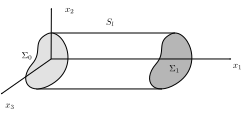
\includegraphics{../images/T1_Ch09-01}
    \end{center}
    \[
        \Omega = [0,l]\times \Sigma
    \]
\end{multicols}
\[
f_i = 0
\]
\begin{equation}
    \left\{
    \begin{aligned}
        S_l:\ [0,l] \times \partial \Sigma & \sigma_{ij} n_j = 0 \\
        \Sigma_0:\ x_1 = 0 & \sigma_{11} = 0 \;,\; u_2 = u_3 = 0 \\
        \Sigma_1:\ x_1 = l & \sigma_{11} = 0 \;,\; u_2 = -\alpha l x_3 \;,\; u_3 = \alpha l x_2
    \end{aligned}
    \right.
    \label{eq:Ch09-033}
\end{equation}

Un CSA $\hat{\sigma}_{ij}$ doit vérifier les équations d'équilibre et les CL de type statique, à savoir
\begin{equation}
    \left\{
    \begin{aligned}
        \hat{\sigma}_{ij} n_j = 0 & \text{sur } [0,l] \times \partial \Sigma \\
        \hat{\sigma}_{11} = 0 & \text{en } x_1= 0 \;,\; x_1=l
    \end{aligned}
    \right.
    \label{eq:Ch09-034}
\end{equation}

Nous inspirant de la solution du paragraphe~\ref{ssec:Ch07-2.2}, nous prenons un champ de contraintes de la forme \eqref{eq:Ch07-048}.
Les CL \eqref{eq:Ch09-034} sur les extrémités sont alors automatiquement vérifiées.
Comme au paragraphe~\ref{ssec:Ch07-2.2}, les équations d'équilibre permettent d'introduire une fonction de contrainte $\Phi$ et les CL \eqref{eq:Ch09-024} sur la surface latérale exigent que $\Phi$ soit nulle sur $\partial \Omega$.
Par contre, pour un CSA, la fonction $\Phi$ ne doit pas vérifier l'êquation~\eqref{eq:Ch07-034} qui résultait des équations de Beltrami.
Ainsi, un CSA est défini par une condition $\hat{\Phi} (x_2, x_3)$ nulle sur $\partial \Sigma$ avec
\begin{equation}
    \hat{\tens{\sigma}} = 
    \begin{bmatrix}
        0 & \hat{\sigma}_{12} & \hat{\sigma}_{13} \\
        \hat{\sigma}_{12} 0 & 0 \\
        \hat{\sigma}_{13} & 0 & 0
    \end{bmatrix}
    \quad , \quad \hat{\sigma}_{12} = \frac{\partial \hat{\Phi}}{\partial x_3} \quad,\quad \hat{\sigma}_{13} = - \frac{\partial \hat{\Phi}}{\partial x_2}
    \label{eq:Ch09-035}
\end{equation}
Pour calculer l'énergie de déformation, en élasticité isotrope, on utitlise les formules suivantes, qui s'obtiennent directement à partir des formules du chapitre~\ref{chap:Ch05}
\begin{align}
    w(\sigma_{ij}) &= w (\varepsilon_{ij}) = \frac{1}{2} \sigma_{ij} \varepsilon_{ij} \\
    &= \frac{1}{2E} \left\{ \sigma_{11}^2 + \sigma_{22}^2 + \sigma_{33}^2 - 2 \nu \left( \sigma_{11} \sigma_{22} - \sigma_{22} \sigma_{33} + \sigma_{33}\sigma_{11} \right) \right\} + \frac{1}{2G} \left( \sigma_{12}^2 + \sigma_{23}^2 + \sigma_{13}^2 \right) \\
    &= \frac{\lambda}{2} \left( \varepsilon_{11} + \varepsilon_{22} + \varepsilon_{33} \right)^2 + 2\mu \left( \varepsilon_{12}^2 + \varepsilon_{23}^2 + \varepsilon_{31}^2 \right)
    \label{eq:Ch09-036}
\end{align}
et à partir de \eqref{eq:Ch09-035} on obtient 
\begin{align}
    \hat{W}\left( \hat{\sigma}_{ij} \right) &= \frac{1}{2G} \iint_{\Sigma} \int_0^l \left\{ \left( \frac{\partial \hat{\Phi}}{\partial x_3} \right)^2 + \left( \frac{\partial \hat{\Phi}}{\partial x_2} \right)^2 \right\} \ud x_1 \ud x_2 \ud x_3 \\
    &= \frac{l}{2G} \iint_{\Sigma} \left\{ \left( \frac{\partial \hat{\Phi}}{\partial x_3} \right)^2 + \left( \frac{\partial \hat{\Phi}}{\partial x_2} \right)^2 \right\} \ud x_2 \ud x_3
    \label{eq:Ch09-037}
\end{align}
Pour calculer $T_u^d$ et $T_f^d$ il faut expliciter la décomposition~\eqref{eq:Ch06-008} pour le problème \eqref{eq:Ch09-033} 
\begin{equation*}
    \begin{aligned}
        \iint_{\partial \Sigma} \sigma_{ij} n_j u_i \ud S &= \iint_{S_l} T_i^d u_i \ud S + \iint_{\Sigma_1} \left[ \sigma_{11}^d u_1 \right. &+ \left. \sigma_{12} u_2^d + \sigma_{13} u_3^d \right] \ud x_2 \ud x_3 \\
        & \underbrace{\phantom{\iint_{S_l} T_i^d u_i \ud S} -\iint_{\Sigma_0} \left[ \sigma_{11}^d u_1 \right.}_{T_f^d (u_i)} &+\underbrace{\left. \sigma_{12} u_2^d + \sigma_{13} u_3^d \right]}_{T_u^d (\sigma_{ij})} \ud x_2 \ud x_3
    \end{aligned}
\end{equation*}
et compte-tenu de la valeur des données \eqref{eq:Ch09-033} 
\begin{equation}
    T_f^d (u_i) = 0
    \label{eq:Ch09-038}
\end{equation}
\begin{equation}
    T_u^d (\hat{\sigma}_{ij}) = \alpha l  \iint_{\Sigma_1} \left( x_2 \hat{\sigma}_{13} - x_3 \hat{\sigma}_{12} \right) \ud x_2 \ud x_3 = \alpha l \hat{\mathcal{M}}_1
    \label{eq:Ch09-039}
\end{equation}
où $\hat{\mathcal{M}}_1$ est le moment de torsion résultant des efforts associés au CSA.
Compte-tenu de \eqref{eq:Ch09-035}, il vient 
\begin{align*}
    T_u^d \left( \hat{\sigma}_{ij} \right) &= - \alpha l \iint_{\Sigma} \left( x_2 \frac{\partial \hat{\Phi}}{\partial x_2} + x_3 \frac{\partial \hat{\Phi}}{\partial x_3} \right) \ud x_2 \ud x_3 \\
    &= 2 \alpha l \iint_{\Sigma} \hat{\Phi} \ud x_2 \ud x_3
\end{align*}
en reprenant le calcul de \eqref{eq:Ch07-063}.
Finalement 
\begin{equation}
    H \left( \hat{\sigma}_{ij} \right) = \iint_{\Sigma} \left\{ 2 \alpha l \hat{\Phi} - \frac{l}{2G} \left[ \left( \frac{\partial \hat{\Phi}}{\partial x_2} \right)^2 + \left( \frac{\partial \hat{\Phi}}{\partial x_3} \right)^2 \right] \right\} \ud x_2 \ud x_3
    \label{eq:Ch09-040}
\end{equation}
ou en posant $\hat{\Phi} = G \alpha \hat{\varphi}$
\begin{equation}
    H \left( \hat{\sigma}_{ij} \right) = \frac{G\alpha^2 l}{2} \iint_{\Sigma} \left\{ 4 \hat{\varphi} - \left( \frac{\partial \hat{\varphi}}{\partial x_2} \right)^2 - \left( \frac{\partial \hat{\varphi}}{\partial x_3} \right)^2 \right\} \ud x_2 \ud x_3
    \label{eq:Ch09-041}
\end{equation}
où $\hat{\varphi}$ est une fonction de $x_2,x_3$ nulle sur $\partial \Sigma$.

Un CCA $\tilde{u}_i$ doit uniquement vérifier les CL de type cinématique 
\begin{equation}
    \left\{
    \begin{aligned}
        \Sigma_0: & \tilde{u}_2 = \tilde{u}_3 = 0 \\
        \Sigma_1: & \tilde{u}_2 = -\alpha l x_3 \quad, \quad \tilde{u}_3 = \alpha l x_2
    \end{aligned}
    \right.
    \label{eq:Ch09-042}
\end{equation}
et, en nous inspirant de la structure \eqref{eq:Ch07-076} de la solution, nous prenons pour CCA le champ 
\begin{equation}
    \tilde{u}_1 = \alpha \tilde{\psi} (x_2, x_3) \quad \tilde{u}_2 = -\alpha x_1 x_3 \quad \tilde{u}_3 = \alpha x_1 x_2
    \label{eq:Ch09-043}
\end{equation}
qui vérifie automatiquement \eqref{eq:Ch09-042}.
Un CCA sera donc défini par une fonction quelconque (effectivement, les restrictions \eqref{eq:Ch07-078} imposées à $\psi$ pour la solution sont d'origine statique).
On a alors
\begin{equation}
    \tilde{\tens{\varepsilon}} = \frac{\alpha}{2}
    \begin{bmatrix}
        0 & -x_3 + \frac{\partial \tilde{\psi}}{\partial x_2} & x_2 + \frac{\partial \tilde{\psi}}{\partial x_3} \\
        -x_3 + \frac{\partial \tilde{\psi}}{\partial x_2} & 0 & 0 \\
        x_2 + \frac{\partial \tilde{\psi}}{\partial x_3} & 0 & 0
    \end{bmatrix}
    \label{eq:Ch09-044}
\end{equation}
et on tire de \eqref{eq:Ch09-036} 
\begin{equation}
    W \left( \tilde{\varepsilon}_{ij} \right) = \frac{G\alpha^2 l}{2} \iint_{\Sigma} \left\{ \left( x_3 - \frac{\partial \tilde{\psi}}{\partial x_2} \right)^2 + \left( x_2 + \frac{\partial \tilde{\psi}}{\partial x_3} \right)^2 \right\}\ud x_2 \ud x_3
    \label{eq:Ch09-045}
\end{equation}
soit finalement, grâce à \eqref{eq:Ch09-038}, 
\begin{equation}
    H \left( \tilde{u}_{i} \right) = \frac{G\alpha^2 l}{2} \iint_{\Sigma} \left\{ \left( x_3 - \frac{\partial \tilde{\psi}}{\partial x_2} \right)^2 + \left( x_2 + \frac{\partial \tilde{\psi}}{\partial x_3} \right)^2 \right\}\ud x_2 \ud x_3
    \label{eq:Ch09-046}
\end{equation}

Ainsi, compte tenu de \eqref{eq:Ch09-046} et \eqref{eq:Ch09-041}, le théorème de comparaison permet d'encadrer $H(u_i) = K(\sigma_{ij})$.
Compte-tenu de \eqref{eq:Ch09-038} et \eqref{eq:Ch09-039}, on a pour la solution 
\begin{equation}
    H(u_i) = K (\sigma_{ij}) = W = \alpha l \mathcal{M}_1 - W = \frac{\alpha l \mathcal{M}_1}{2} = \frac{G\alpha^2 l}{2} I    
    \label{eq:Ch09-047}
\end{equation}
compte-tenu de \eqref{eq:Ch07-064}.
Le théorème de comparaison nous donne donc 
\begin{equation}
    \left\{
    \begin{aligned}
        & h \left( \hat{\varphi} \right) \leq I \leq k \left( \tilde{\psi} \right) \\
        & h \left( \hat{\varphi} \right) = \iint_{\Sigma} \left\{ 4 \hat{\varphi} - \left( \frac{\partial \hat{\varphi}}{\partial x_2} \right)^2 - \left( \frac{\partial \hat{\varphi}}{\partial x_3} \right)^2 \right\} \ud x_2 \ud x_3 \\
        & k \left( \tilde{\psi} \right) = \iint_{\Sigma} \left\{ \left( x_3 - \frac{\partial \tilde{\psi}}{\partial x_2} \right)^2 + \left( x_2 + \frac{\partial \tilde{\psi}}{\partial x_3} \right)^2 \right\} \ud x_2 \ud x_3
    \end{aligned}
    \right.
    \label{eq:Ch09-048} 
\end{equation}
valable pour toute fonction $\hat{\varphi}$ nulle sur $\partial \Sigma$ et toute fonction $\tilde{\psi}$.
On voit donc que l'on peut encadrer le module de rigidité à la torsion et obtenir ainsi des valeurs approchées. 

On peut ainsi démontrer certains résultats généraux: par exemple, en prenant $\tilde{\psi} = 0$ on obtient
\begin{equation}
    I \geq \iint_{\Sigma} \left( x_2^2 + x_3^2 \right) \ud x_2 \ud x_3 = I_0
    \label{eq:Ch09-049}
\end{equation}
le moment polaire $I_0$ est un minorant du module de rigidité à la torsion (on a vu que c'était le module de rigidité à la torsion pour une section circulaire ou annulaire). 

Pour aller plus loin, considérons par exemple le cas d'une section rectangulaire.
On a vu au paragraphe~\ref{ssec:Ch07-2.4} que l'on pouvait obtenir une solution exacte par développement en série de Fourier.
Les calculs précédents vont nous fournir une valeur approchée.
La fonction $\hat{\varphi}$ doit être nulle sur le bord, nous prenons 
\begin{equation}
    \hat{\varphi} = m (a^2 - x_2^2) (b^2 -x_3^2)
    \label{eq:Ch09-050}
\end{equation}
On trouve alors par un calcul direct 
\begin{equation}
    h\left( \hat{\varphi} \right) = \frac{64 a^3 b^3}{9} m \left[ 1 - \frac{2m}{5}\left( a^2 + b^2 \right) \right]
    \label{eq:Ch09-051}
\end{equation}
La fonction $\tilde{\psi}$ est quelconque par analogie avec la section elliptique, nous prenons 
\begin{equation}
    \tilde{\psi} = p x_2 x_3
    \label{eq:Ch09-052}
\end{equation}
et nous obtenons 
\begin{equation}
    k\left( \tilde{\psi} \right) = \frac{4 ab}{3} \left[ (p+1)^2 b^2 + (p-1)^2 a^2 \right]
    \label{eq:Ch09-053}
\end{equation}
d'où l'encadrement \eqref{eq:Ch09-048} pour $I$.
Pour obtenir l'encadrement optimal, nous choisissons la valeur de $m$ qui maximise $h(\hat{\varphi})$ et la valeur de $p$ qui minimise $k(\tilde{\psi})$.
On trouve 
\[
m_{opt} = \frac{5}{4\left( a^2 + b^2\right)} \quad p_{opt} = \frac{a^2-b^2}{a^2+b^2}
\]
\begin{equation}
    \frac{40}{9} \frac{a^3 b^3}{a^2 + b^2} \leq I \leq \frac{48}{9} \frac{a^3 b^3}{a^2 +b^2}
    \label{eq:Ch09-054}
\end{equation}
En particulier pour la section carrée, on trouve 
\begin{equation}
    0,139 \leq \frac{I}{a^4} \leq 0,167
    \label{eq:Ch09-055}
\end{equation}
alors que la valeur exacte est de 0,141.
Bien entendu, on pourrait raffiner en prenant des fonctions $\hat{\varphi}$ et $\tilde{\psi}$ plus compliquées.
Néanmoins, on voit que notre CSA est déjà assez proche de la solution, et peut nous donner une approximation raisonnable du champ de contraintes réel. 

\section{Les théorèmes de l'énergie} \label{sec:Ch09-2}
\subsection{Le théorème de réciprocité} \label{ssec:Ch09-2.1}
On considère un solide élastique pouvant être soumis à deux chargements différents.
Soit $\left( u_i^1, \sigma_{ij}^1 \right)$ et $\left( u_i^2, \sigma_{ij}^2 \right)$ les solutions correspondantes.

\newtheorem*{ThMB}{Théorème de réciprocité au de Maxwell-Betti}
\begin{ThMB}
    Le travail des efforts extérieurs $2$ dans le déplacement $1$ est égal au travail des efforts extérieurs $1$ dans le déplacement $2$.
    \begin{equation}
        \iint_{\Omega} f_i^2 u_i^1 \ud v + \iint_{\partial \Omega} T_i^2 u_i^1 \ud S = \iiint_{\Omega} f_i^1 u_i^2 \ud v + \iint_{\partial \Omega} T_i^1 u_i^2 \ud S
        \label{eq:Ch09-056}
    \end{equation}
\end{ThMB}
\begin{proof}
    On utilise le théorème des travaux virtuels appliqué au problème 1 avec comme déplacement virtuel le déplacement $u_i^2$ solution du problème 2. 
    On obtient
    \begin{displaymath}
        \iiint_{\Omega} \sigma_{ij}^1 \varepsilon_{ij}^2 \ud v = \iiint_{\Omega} f_i^1 u_i^2 \ud v + \iint_{\partial \Omega} T_i^1 u_i^2 \ud S
    \end{displaymath}
    On effectue la même opération en changeant 1 et 2 
    \begin{displaymath}
        \iiint_{\Omega} \sigma_{ij}^2 \varepsilon_{ij}^1 \ud v = \iiint_{\Omega} f_i^2 u_i^1 \ud v + \iint_{\partial \Omega} T_i^2 u_i^1 \ud S
    \end{displaymath}
    et on obtient \eqref{eq:Ch09-056} en remarquant que d'après la symétrie de la matrice d'élasticité 
    \begin{displaymath}
        \iiint_{\Omega} \sigma_{ij}^2 \varepsilon_{ij}^1 \ud v = \iiint_{\Omega} A_{ijkh} \varepsilon_{ij}^1 \varepsilon_{kh}^2 \ud v = \iiint_{\Omega} \sigma_{ij}^1 \varepsilon_{ij}^2 \ud v
    \end{displaymath}
\end{proof}

A titre d'exemple d'application, considérons un problème du type II avec des données $\left( f_i, T_i^d \right)$.
En général, on ne saura pas calculer la solution $\left( u_i, \sigma_{ij} \right)$.
Par contre, certains problèmes de type II peuvent être résolus pour le même domaine, par exemple teus ceux qui admettent une solution homogène: le problème caractérisé par les données 
\begin{equation}
    f_i = 0 \quad T_i^d = \sigma_{ij}^0 n_j
    \label{eq:Ch09-057}
\end{equation}
où $\sigma_{ij}^0$ est constant, admet en effet la solution 
\begin{equation}
    \sigma_{ij} = \sigma_{ij}^0 \quad u_i = \Lambda_{ijkh} \sigma_{kh}^0 x_j
    \label{eq:Ch09-058}
\end{equation}

On applique le théorème de Maxwell Betti en prenant comme problème I  le problème posé, et comme problème 2 le problème \eqref{eq:Ch09-057} avec sa solution \eqref{eq:Ch09-058}:
\[
\iint_{\partial \Omega} \sigma_{ij}^0 n_j u_i \ud S = \iiint_{\Omega} \Lambda_{ijkh} \sigma_{kh}^0 x_j f_i \ud v + \iint_{\partial \Omega} \Lambda_{ijkh} \sigma_{kh}^0 x_j T_i^d \ud S
\]
Mais l'utilisation du théorème de la divergence donne 
\[
\iint_{\partial \Omega} \sigma_{ij}^0 n_j u_i \ud v = \sigma_{ij}^0 \iiint_{\Omega} \varepsilon_{ij} \ud v
\]
et \eqref{eq:Ch09-058} donne des informations sur la valeur moyenne des déformations 
\begin{equation}
    \sigma_{ij}^0 \iiint_{\Omega} \varepsilon_{ij} \ud v = \iiint_{\Omega} \Lambda_{ijkh} \sigma_{kh}^0 x_j f_i \ud v + \iint_{\partial \Omega} \Lambda_{ijkh} \sigma_{kh}^0 x_j T_i^d \ud S
    \label{eq:Ch09-059}
\end{equation}
Par exemple, on obtiendra la valeur moyenne de $\varepsilon_{11}$ et $\varepsilon_{12}$ en prenant pour $\sigma_{ij}^0$ un tenseur de traction simple et de cisaillement simple.
En élasticité isotrope on obtient
\begin{equation}
    \left\{
    \begin{aligned}
        \frac{1}{V} \iiint_{\Omega} \varepsilon_{11} \ud v &= \frac{1}{V} \frac{1}{E} \left\{ \iiint_{\Omega} \left[ f_1 x_1 - \nu \left( f_2 x_2 + f_3 x_3 \right) \right] \ud v + \iint_{\partial \Omega} \left[ T_1^d x_1 - \nu \left( T_2^d x_2 + T_3^d x_3 \right) \right] \ud S \right\} \\
        \frac{1}{V} \iiint_{\Omega} \varepsilon_{12} \ud v &= \frac{1}{V} \frac{1+ \nu}{E} \left\{ \iiint_{\Omega} \left( f_1 x_2 + f_2 x_1 \right) \ud v + \iint_{\partial \Omega} \left( T_1^d x_2 + T_2^d x_1 \right) \ud S \right\}
    \end{aligned}
    \right.
    \label{eq:Ch09-060}
\end{equation}
En particulier, la variation de volume est donnée par 
\begin{equation}
    \Delta V = \iiint_{\Omega} \varepsilon_{ii} \ud v = \frac{1}{3\lambda+2\mu} \left\{ \iiint_{\Omega} f_i x_i \ud v + \iint_{\partial \Omega} T_i^d x_i \ud S \right\}
    \label{eq:Ch09-061}
\end{equation}
Plus généralement, le théorème de Maxwell Betti permet souvent d'obtenir sans calcul des résultats intéressants. 

\subsection{Le théorème de Castigliano} \label{ssec:Ch09-2.2}
On considère encore le même solide élastique pouvant être soumis à deux systèmes de chargements 1 et 2. 
\newtheorem*{ThCast}{Théorème de Castigliano}
\begin{ThCast}
    Soit $\hat{\sigma}_{ij}^2$ un CSA pour le problème 2.
    Le travail des efforts extérieurs 2 dans le déplacement 1 est égal à la dérivée à l'origine de la fonction donnant l'énergie de déformation du champ de contraintes $\sigma_{ij}^1 + \lambda \hat{\sigma}_{ij}^2$ en fonction de $\lambda$.
    \begin{equation}
        \iiint_{\Omega} f_i^2 u_i^1 \ud v + \iint_{\partial \Omega} T_i^2 u_i^1 \ud S = \frac{\ud}{\ud \lambda} \left\{ \hat{W}\left( \sigma_{ij}^1 + \lambda \hat{\sigma}_{ij}^2 \right) \right\} |_{\lambda=0}
        \label{eq:Ch09-062}
    \end{equation}
\end{ThCast}
\begin{proof}
    On développe 
    \[
    \hat{W}\left( \sigma_{ij}^1 + \lambda \hat{\sigma}_{ij}^2 \right) = \hat{W} \left( \sigma_{ij}^1 \right) + \lambda^2 \hat{W}\left( \hat{\sigma}_{ij}^2 \right) + \lambda \iiint_{\Omega} \Lambda_{ijkh} \sigma_{ij}^1 \hat{\sigma}_{kh}^2 \ud v
    \]
    De sorte que 
    \begin{align*}
    \frac{\ud}{\ud \lambda} \left\{ \hat{W}\left( \sigma_{ij}^1 + \lambda \hat{\sigma}_{ij}^2 \right) \right\} |_{\lambda=0} &= \iiint_{\Omega} \Lambda_{ijkh} \sigma_{ij}^1 \hat{\sigma}_{kh}^2 \ud v \\
        &= \iiint_{\Omega} \varepsilon_{kh}^1 \hat{\sigma}_{kh}^2 \ud v \\
        &= \iiint_{\Omega} f_i^2 u_i^1 \ud v + \iint_{\partial \Omega} T_i^2 u_i^1 \ud v
    \end{align*}
\end{proof}

L'utilisation de ce théorème et du théorème de réciprocité est basée sur le fait que, en introduisant comme chargement 2 des chargements fictifs, ils permettent de calculer certains déplacements ou déformations.
En effet, si on introduit par exemple comme chargement 2 une force concentrée $\vec{F}$ appliquée au point $M$, alors le travail du  chargement 2 dans le déplacement 1 se réduit à
\begin{equation}
    \vec{F}\cdot \vec{u}^1 \left( M\right)
    \label{eq:Ch09-063}
\end{equation}
d'où le calcul du 9éplacement du point $M$ pour le problème 1.
Ce type de méthode est peu utilisé en MMC, pour deux raisons: 
\begin{enumerate}
    \item L'introduction de forces concentrées en MMC pose quelques problèmes liés à la singularité du chargement.
        On sait résoudre ces problèmes, mais ce n'est pas si simple. 
    \item En MMC, il est en général très difficile de calculer le champ de contraintes solution ou de construire un CSA. 
\end{enumerate}

Par contre, ces «~théorèmes de l'énergie~» -- comme sont couramment nommés le théorème de réciprocité et le théorème de Castigliano --seront utilisés de manière intensive en Résistance des Matériaux, où les deux difficultés mentionnées ci-dessus disparaissent.
De manière générale en effet, tous les théorèmes que nous avons démontrés depuis le début de ce chapitre sont valables pour toute théorie des milieux continus élastiques.
En fait, ils reposent sur la structure algébrique décrite à la fin du paragraphe~\ref{ssec:Ch09-1.1}.

Ces théorèmes ne sont en principe valables que pour les problèmes réguliers.
Pour un problème non régulier -- problème avec frottement ou avec contact unilatéral par exemple, voir paragraphe~\ref{ssec:Ch06-1.1} -- on peut avoir des résultats analogues, mais il convient de tout reprendre pour chaque cas particulier.
C'est le champ d'étude des méthodes variationnelles (\cite{Duvaut-72}). 

\section{La méthode des éléments finis} \label{sec:Ch09-3}
\subsection{Principe de la méthode} \label{ssec:Ch09-3.1}
Les théorèmes du paragraphe~\ref{sec:Ch09-1} énoncent des principes variationnels dont l'affirmation type est la suivante: «~La solution minimise une certaine fonctionnelle dans un espace de fonctions admissibles~».
Nous avons présenté les deux principes variationnels traditionnels, mais il en existe bien d'autres, plus ou moins appropriés, suivant le type de problème que l'on envisage~\cite{Valid-77}.
L'intérêt de ces principes variationnels réside dans le fait qu'ils engendrent à peu près automatiquement une méthode numérique pour calculer une solution approchée.
Il suffit en effet de discrétiser l'espace des fonctions admissibles -- c'est à dire de l'approcher par un espace de dimension finie -- et de minimiser la fonctionnelle sur cet espace discrétisé.
On obtient ainsi une solution approchée d'autant plus proche de la solution réelle que l'espace discrétisé approche mieux l'espace des fonctions admissibles. 

Pour discrétiser l'espace des fonctions admissibles, on peut par exemple introduire une base fonctionnelle de cet espace -- base de fonctions sinusoïdales pour un domaine rectangulaire, par exemple -- et approcher l'espace des fonctions admissibles par l'espace engendré par les $n$ premiers éléments de cette base. 
C'est la méthode de Galerkin, et on peut montrer que lorsque $n\rightarrow\infty$, la solution approchée ainsi calculée tend vers la solution réelle. 

Le terme «~méthode d'éléments finis~» recouvre un ensemble de méthodes pour lesquelles l'espace discrétisé s'obtient 
\begin{enumerate}
    \item en découpant le domaine $\Omega$ en un certain nombre de sous-domaines simples (triangles ou rectangles): les éléments finis; 
    \item en prenant sur chaque élément une forme analytique simple, de sorte que la valeur de la fonction en tout point est donnée par sa valeur en un nombre limité de nœuds.
\end{enumerate}
A titre d'exemple, nous allons présenter les trois éléments les  plus simples pour un espace de fonctions à valeur scalaire  (pour une fonction à valeur vectorielle ou tensorielle, il suffit de  considérer séparément chaque composante) dans le plan.  

\paragraph{Exemple 1.}
\begin{multicols}{2}
Elément triangulaire avec fonction linéaire sur chaque triangle 
\[
f = a +b x_1+cx_2
\]
La valeur de la fonction $f$ en un point du triangle ABC dépend de 3 paramètres, par exemple la valeur de $f$ aux trois sommets 
\columnbreak
\begin{center}
    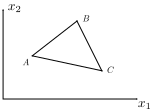
\includegraphics{../images/T1_Ch09-02}
\end{center}
\end{multicols}
\begin{equation}
    f = f_A \lambda_A (x_1,x_2) + f_B \lambda_B (x_1,x_2) + f_C \lambda_C (x_1, x_2)
    \label{eq:Ch09-064}
\end{equation}
où $\lambda_A$, $\lambda_B$, $\lambda_C$ sont les «~coordonnées barycentriques~» du point $M$. 

\paragraph{Exemple 2.} 
\begin{multicols}{2}
Elément rectangulaire avec fonction bilinéaire 
\[
f = a +b x_1+cx_2 +dx_1x_2
\]
La valeur de la fonction $f$ en un point $M$ du rectangle ABCD dépend de 4 paramètres: la valeur $f$ aux nœuds A, B, C, D. 
\columnbreak
\begin{center}
    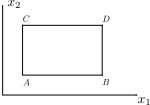
\includegraphics{../images/T1_Ch09-03}
\end{center}
\end{multicols}
\begin{multline}
    f = f_A \frac{(x_1 - x_1^B)(x_2 -x_2^C)}{(x_1^A - x_1^B)(x_2^A-x_2^C)} +  f_B \frac{(x_1 - x_1^A)(x_2 -x_2^D)}{(x_1^B - x_1^A)(x_2^B-x_2^B)} \\
    + f_C \frac{(x_1 - x_1^D)(x_2 -x_2^A)}{(x_1^C - x_1^D)(x_2^C-x_2^A)} + f_D \frac{(x_1 - x_1^C)(x_2 -x_2^B)}{(x_1^D - x_1^C)(x_2^D-x_2^B)}
    \label{eq:Ch09-065} 
\end{multline}

\paragraph{Exemple 3.}
\begin{multicols}{2}
Elément triangulaire avec fonction quadratique sur chaque triangle 
\begin{equation}
    f = a + b x_1 + c x_2 + d x_1^2 + e x_1 x_2 +f x_2^2
    \label{eq:Ch09-066}
\end{equation}
La valeur de la fonction sur le triangle ABC dépend de 6 paramètres: la valeur de $f$ aux 6 nœuds A, B, C, D, E, F, et ainsi de suite.
On trouvera dans la littérature sur les éléments finis des «~catalogues~» d'éléments. 
\columnbreak
\begin{center}
    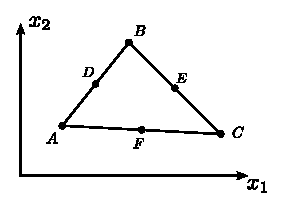
\includegraphics{../images/T1_Ch09-04}
\end{center}
\end{multicols}
Après avoir découpé le modèle et choisi les éléments, une fonction de l'espace discrétisé est définie par sa valeur en un certain nombre de nœuds, et on doit minimiser une fonction d'un nombre fini de variables, problème qui se prête bien au calcul numérique. 

Pour la torsion, par exemple, on peut à partir de \eqref{eq:Ch09-048} construire méthodes d'éléments finis
\begin{description}
    \item[1ère méthode.] On discrétise $\Sigma$, et on maximise la fonctionne11e $h(\hat{\varphi})$ sur l'espace des fonctions $\hat{\varphi}$ nulles sur le bord. 
    \item[2ème méthode.] On discrétise $\Sigma$, et on minimise la fonctionnelle $h(\hat{\psi})$ sur l'espace de toutes les fonctions $\hat{\psi}$.
\end{description}

\subsection{Application à un exemple} \label{ssec:Ch09-3.2}
Pour montrer la mise en œuvre de la méthode, nous allons envisager un exemple.
Considérons en déformations planes un barrage triagulaire OAB
\begin{center}
    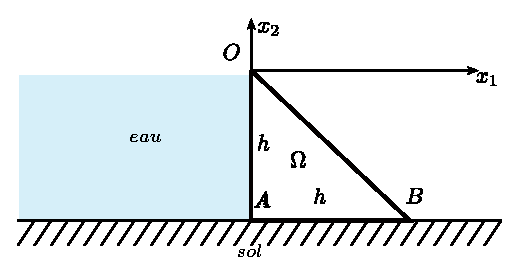
\includegraphics{../images/T1_Ch09-05}
\end{center}
Les forces de volume se réduisent à la pesanteur 
\begin{equation}
    f_1 = 0 \quad,\quad f_2 = -\rho g
    \label{eq:Ch09-067}
\end{equation}
$\rho$ étant la masse volumique du béton.
Quant aux conditions aux limites, elles traduisent l'absence de contrainte sur OB, l'effet de la pression hydrostatique $-\varpi x_2$ ($\varpi$ étant le poids spécifique de l'eau) sur OA, et la liaison supposée rigide avec le sol sur AB 
\begin{equation}
    \left\{
    \begin{aligned}
        \text{OB} & \sigma_{11} + \sigma_{12} = 0 \quad,\quad \sigma_{12} + \sigma_{22} = 0 \\
        \text{OA} & \sigma_{11} = \varpi x_2 \quad,\quad \sigma_{12} = 0 \\
        \text{AB} & u_1 = u_2 = 0
    \end{aligned}
    \right.
    \label{eq:Ch09-068}
\end{equation}

Le théorème de l'énergie potentielle affirme que dans l'espace des CCA, 
\begin{equation}
    \mathcal{U} = \left\{ \left( \tilde{u}_1, \tilde{u}_2 \right) | \tilde{u}_1 = \tilde{u}_2 = 0 \text{ pour } x_2 = -h \right\}
    \label{eq:Ch09-069}
\end{equation}
la solution minimise la fonctionnelle 
\begin{equation}
    K\left( \tilde{u}_i \right) = \frac{1}{2} \iint_{\Omega} A_{ijkh} \tilde{\varepsilon}_{ij} \tilde{\varepsilon}_{kh} \ud x_1 \ud x_2 + \iint_{\Omega} \rho g \tilde{u}_2 \ud x_1 \ud x_2 + \int_{\text{OA}} \varpi x_2 \tilde{u}_1 \ud x_2
    \label{eq:Ch09-070}
\end{equation}

Pour discrétiser ce problème, nous introduisons un découpage en éléments finis 
\begin{center}
    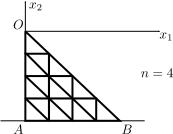
\includegraphics{../images/T1_Ch09-07}
\end{center}
Par exemple, nous introduisons un maillage régulier et des éléments triangulaires du type \eqref{eq:Ch09-064}, et nous approchons $\mathcal{U}$ par
\[
\mathcal{U}_n = \left\{ \left( u_1, u_2 \right),\ u_1 \text{ et } u_2\ \text{nuls sur AB et de la forme~\eqref{eq:Ch09-064} sur chaque triangle} \right\}
\]
Ainsi, une fonction de $\mathcal{U}_n$ sera caractérisée par sa valeur aux $n(n+1)/2$ points du maillage non situés sur AB (si OA et AB sont découpés en $n$ intervalles égaux).
Ainsi, l'espace $\mathcal{U}_n$ est un espace de dimension $n(n+1)$, et une fonction de $\mathcal{U}_n$ sera caractérisée par un vecteur colonne $\underline{U}$ de $n(n+1)$ éléments donnant les deux composantes de $u_i$ en chaque point du maillage, la formule \eqref{eq:Ch09-064} donnant alors la valeur de $u_i$ en tout point.
Si l'on reporte cette fonction dans la définition \eqref{eq:Ch09-070} ou \eqref{eq:Ch09-015} de l'énergie potentielle, l'énergie de déformation $W\left( \tilde{\varepsilon}_{ij} \right)$ devient une forme quadratique par rapport aux composantes de $\underline{U}$ et le travail des efforts $\tilde{T}_f^d$ devient une forme linéaire par rapport à ces mêmes composantes.
Ainsi 
\begin{equation}
    K \left( \tilde{u}_i \right) = \frac{1}{2} \underline{U}^T \underline{\underline{\mathcal{A}}} \underline{\underline{U}} - \underline{F}^T \underline{U}
    \label{eq:Ch09-071}
\end{equation}
où la matrice carrée $\underline{\underline{A}}$ est la matrice de rigidité, symétrique et définie positive, et où le vecteur colonne $\underline{F}$ caractérise les efforts extérieurs.
Pour minimiser l'énergie potentielle, il faut donc résoudre le système 
linéaire 
\begin{equation}
    \underline{\underline{A}} \underline{U} = \underline{F}
    \label{eq:Ch09-072}
\end{equation}
Nous utilisons ici le théorème de l'énergie potentielle, car en 
MMC il est en général très difficile d'engendrer des champs statiquement admissibles, et le théorème de l'énergie complémentaire est peu utilisé dans ce contexte. 
\subsection{Étude d'un élément} \label{ssec:Ch09-3.3}
Pour calculer les intégrales qui interviennent dans \eqref{eq:Ch09-070}, il faudra sonnner les contributions de chaque triangle pour les intégrales de sur face, et de chaque segment pour les intégrales de ligne.
Nous allons donc déjà examiner la contribution d'un élément triangulaire abc à l'énergie de déformation au travail des efforts de volume, et au travail des efforts de surface. 

Sur chaque élément, nous pouvons donc écrire le déplacement en fonction de la valeur aux sommets a, b et c de cet élément 
\begin{equation}
    \tilde{u}_i = u_i^a \lambda_a \left( x_1, x_2 \right) + u_i^b \lambda_b \left( x_1, x_2 \right) + u_i^c \lambda_c \left( x_1, x_2 \right)
    \label{eq:Ch09-073}
\end{equation}
où $\lambda_a$, $\lambda_b$ et $\lambda_c$ sont les coordonnées barycentriques du point définies par 
\begin{equation}
    \begin{bmatrix}
        \lambda_a\\
        \lambda_b\\
        \lambda_c
    \end{bmatrix}
    =
    \begin{bmatrix}
        1 & 1 & \\
        x_1^a & x_1^b & x_1^c \\
        x_2^a & x_2^b & x_2^c
    \end{bmatrix}^{-1}
    \begin{bmatrix}
        1 \\
        x_1 \\
        x_2
    \end{bmatrix}
    \label{eq:Ch09-074}
\end{equation}
et qui dépendent uniquement de la géométrie de l'élément.
\eqref{eq:Ch09-073} donne donc
\begin{equation}
    \begin{bmatrix}
        \tilde{u}_1 \\
        \tilde{u}_2
    \end{bmatrix}
    \begin{bmatrix}
        u_1^a & u_1^b & u_1^c \\
        u_2^a & u_2^b & u_2^c
    \end{bmatrix}
    \begin{bmatrix}
        1 & 1 & \\
        x_1^a & x_1^b & x_1^c \\
        x_2^a & x_2^b & x_2^c
    \end{bmatrix}^{-1}
    \begin{bmatrix}
        1 \\
        x_1 \\
        x_2
    \end{bmatrix}
    \label{eq:Ch09-075}
\end{equation}
\subsubsection{Discrétisation de l'énergie.}
Le tenseur des déformations $\varepsilon_{ij}$ est alors constant et donné par
\begin{equation}
    \begin{bmatrix}
        \varepsilon_{11} & \varepsilon_{12} \\
        \varepsilon_{12} & \varepsilon_{22}
    \end{bmatrix}
    =
    \left\{ 
    \begin{bmatrix}
        u_1^a & u_1^b & u_1^c \\
        u_2^a & u_2^b & u_2^c
    \end{bmatrix}
    \begin{bmatrix}
        1 & 1 & \\
        x_1^a & x_1^b & x_1^c \\
        x_2^a & x_2^b & x_2^c
    \end{bmatrix}^{-1}
    \begin{bmatrix}
        0 & 0 \\
        1 & 0 \\
        0 & 1
    \end{bmatrix}
    \right\}^S
    \label{eq:Ch09-076}
\end{equation}
où $\underline{\underline{A}}^S$ désigne la matrice $\underline{\underline{A}}$ symétrisée
\begin{equation}
    \underline{\underline{A}}^S = \frac{1}{2} \left( \underline{\underline{A}} + \underline{\underline{A}}^T \right)
    \label{eq:Ch09-077}
\end{equation}
L'intégration de l'énergie de déformation sur le triangle abc donne
\begin{equation}
    \begin{aligned}
        W_{abc} &= \frac{1}{2} \iint_{abc} \left\{ \lambda \left( \varepsilon_{11} + \varepsilon_{22} \right)^2 + 2 \left( \varepsilon_{11}^2 + \varepsilon_{22}^2 + 2 \varepsilon_{12}^2 \right) \right\} \ud x_2 \ud x_2
        &= \frac{1}{2} \underline{u}^T \underline{\underline{a}}_{abc} \underline{u}
    \end{aligned}
    \label{eq:Ch09-078}
\end{equation}
où $\underline{u}$ désigne le vecteur colonne des déplacements  aux nœuds, donc un sous-vecteur de $\underline{U}$, et où $\underline{\underline{a}}_{abc}$ est une matrice symétrique $6\times6$ qui résulte de l'intégration sur le triangle et il dépend donc uniquement de la géométrie.

Si l'on dérive la forme qui \tmp{ itit } $W_{abc}$ par rapport aux déplacements des nœuds, on obtient un vecteur colonne
\begin{multicols}{2}
    \begin{center}
        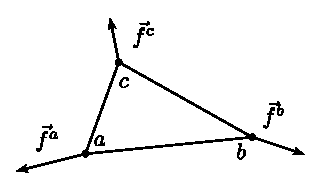
\includegraphics{../images/T1_Ch09-08}
    \end{center}
    \columnbreak
\begin{equation}
    f = \underline{\underline{a}}_{abc} \underline{u} = \frac{\partial W_{abc}}{\partial \underline{u}}
    \label{eq:Ch09-079}
\end{equation}
qui peut s'interpréter énergétiquement comme donnant les «~forces élastiques $\vec{f}^a$, $\vec{f}^b$, $\vec{f}^c$~», qui doivent être appliquées aux nœuds pour produire le déplacement $\underline{u}$.
\end{multicols}
Ceci résulte par exemple du bilan énergétique \eqref{eq:Ch09-032} qui montre que pour une variation $\ud \underline{u}$ des déplacements aux nœuds, la variation de l'énergie de déformation 
\begin{equation}
    \ud W_{abc} = \underline{f}^T \ud u
    \label{eq:Ch09-080}
\end{equation}
est égale au travail des efforts exercés sur l'élément.
On peut donc interpréter \eqref{eq:Ch09-080} comme donnant le travail des «~forces élastiques~» (suppoées concentrées aux nœuds) $\vec{f}^a$, $\vec{f}^b$, $\vec{f}^c$.
Il faut bien garder à l'esprit, cependant, qu'il ne s'agit là que d'une interprétation, et que ces «~forces élastiques~» sont fictives et sans aucune existence réelle; ce ne sont pas 
des forces, mais des dérivées de l'énergie de déformation. 

\subsubsection{Discrétisation des forces de volume}
Calculons la contribution du triangle abc au travail des forces de volume, c'est à dire dans \eqref{eq:Ch09-070} des forces de pesanteur.
En reportant \eqref{eq:Ch09-073} dans \eqref{eq:Ch09-070} et en remarquant que 
\begin{equation}
    \iint_{abc} \lambda_a \ud x_1 \ud x_2 = \iint_{abc} \lambda_b \ud x_1 \ud x_2 = \iint_{abc} \lambda_c \ud x_1 \ud x_2 = \frac{S}{3}
    \label{eq:Ch09-081}
\end{equation}
on obtiendra
\begin{equation}
    -\iint_{abc} \rho g \tilde{u}_2 \ud x_1 \ud x_2 = - \frac{\rho g S}{3} \left( u_2^a + u_2^b + u_2^c \right) = \underline{\varphi}^T \cdot \underline{u}
    \label{eq:Ch09-082}
\end{equation}
\begin{equation}
    \underline{\varphi}^T = \left( 0, 0, 0, -\frac{\rho g S}{3}, -\frac{\rho g S}{3}, -\frac{\rho g S}{3} \right)
    \label{eq:Ch09-083}
\end{equation}
D'un point de vue énergétique, on peut interpréter \eqref{eq:Ch09-082} en disant que les forces de volume sont équivalentes aux trois forces concentrées $\vec{\varphi}^a$, $\vec{\varphi}^b$, $\vec{\varphi}^c$ appliquées aux nœuds. 
\begin{center}
    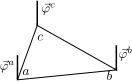
\includegraphics{../images/T1_Ch09-09}
\end{center}
De manière générale, l'écriture du travail des efforts de volume conduit à décomposer ces efforts en trois forces concentrées appliquées aux nœuds. 

\subsubsection{Discrétisation des efforts surfaciques}
Soit ac un côté du triangle abc appartenant à $S_f$, c'est à dire où les efforts surfaciques sont donnés
\begin{multicols}{2}
    \begin{center}
        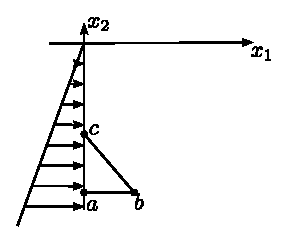
\includegraphics{../images/T1_Ch09-10}
    \end{center}
    \begin{center}
        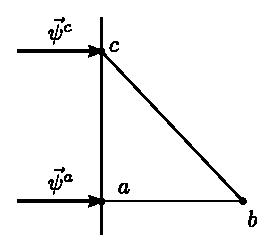
\includegraphics{../images/T1_Ch09-11}
    \end{center}
\end{multicols}
La restriction de \eqref{eq:Ch09-075} à ac donne, dans le cas particulier du barrage (ac vertical) 
\begin{equation}
    \tilde{u}_1 = u_1^a \frac{x_2 - x_2^c}{x_2^a -x_2^c} + u_1^c \frac{x_2 - x_2^a}{x_2^c -x_2^a}
    \label{eq:Ch09-084}
\end{equation}
De sorte que la contribution de ac au travail des efforts surfaciques est 
\[
\frac{\varpi}{x_2^c -x_2^a} \int_{x_2^a}^{x_2^c} \left[ u_1^c x_2 \left( x_2 - x_2^a \right) - u_1^a x_2 \left( x_2 - x_2^c \right) \right] \ud x_2
\]
et on obtient finalement
\begin{equation}
    - \int_{a}^c \varpi x_2 \tilde{u}_1 \ud x_2 = - \frac{\varpi \Delta h}{2} \left[ \left( x_2^c - \frac{\Delta h}{3} \right) u_1^c + \left( x_2^a + \frac{\Delta h}{3} \right) u_2^c \right]
    \label{eq:Ch09-085}
\end{equation}
\begin{equation}
    \underline{\psi}^T = \left( - \frac{\varpi \Delta h \left( x_2^c + \frac{\Delta h}{3} \right)}{2}, 0, - \frac{\varpi \Delta h \left( x_2^a - \frac{\Delta h}{3} \right)}{2}, 0, 0, 0 \right)
    \label{eq:Ch09-086}
\end{equation}

D'un point de vue énergétique, les forces de contact exercées sur  ac sont équivalentes à deux forces concentrees  $\vec{\psi}^a$ et $\vec{\psi}^c$ exercées aux nœuds.
Par contre,  $u_i^b$ n'intervient pas dans \eqref{eq:Ch09-084}, et donc $\vec{\psi}^b=0$.

\subsection{Assemblage} \label{ssec:Ch09-3.4}
Pour calculer $K \left( \tilde{u}_i \right)$, c'est à dire pour expliciter \eqref{eq:Ch09-071}, on doit sommer la contribution de tous les triangles pour l'énergie de déformation et le travail des forces de volume, ainsi que la contribution de tous les segments de $S_f$ pour le travail des forces de surface.
Pour minimiser la fonction $K\left( \underline{U} \right)$ résultante, il faut annuler la dérivée de $K$ par rapport à chaque déplacement de chaque nœud. 
\subsubsection{Cas d'un nœud intérieur a}
\begin{multicols}{2}
    \begin{center}
        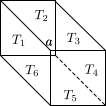
\includegraphics{../images/T1_Ch09-12}
    \end{center}
    \columnbreak
Chaque nœud intérieur appartient à $n$ triangles $T_1,\ T_2, \cdots T_n$ ($n=6$ dans notre exemple).
D'après ce qu'on a vu au paragraphe précédent, le déplacement $u_i^ a$ n'interviendra dans $K$ que par la contribution de ces $n$ triangles.
\end{multicols}
On pourra donc écrire 
\begin{equation}
    \frac{\partial W}{\partial u_i^a} = \frac{\partial W_{T_1}}{\partial u_i^a} + \cdots + \frac{\partial W_{T_n}}{\partial u_i^a} = f_i^{a,T_1} + \cdots + f_i^{a, T_n}
    \label{eq:Ch09-087}
\end{equation}
où les quantités $f_i^{a,T_j}$ sont les composantes des forces élastiques appliquées en a sur chacun des éléments  $T_1,\ T_2, \cdots T_n$ entourant a.
\begin{equation}
    \begin{aligned}
        \frac{\partial }{\partial u_1^a} \iint_{\Omega} \rho g \tilde{u}_2 \ud x_1 \ud x_2 &= 0 = - \left( \varphi_1^{a,T_1} + \cdots + \varphi_1^{a,T_n} \right) \\
        \frac{\partial }{\partial u_2^a} \iint_{\Omega} \rho g \tilde{u}_2 \ud x_1 \ud x_2 &= \frac{\rho g}{3} \left( S^1 + \cdots + S^n \right) = - \left( \varphi_2^{a,T_1} + \cdots + \varphi_2^{a,T_n} \right)
    \end{aligned}
    \label{eq:Ch09-088}
\end{equation}
où les quantités $\varphi_i^{a,T_j}$ sont les forces concentrées en a équivalentes aux forces de volume exercées sur chacun des éléments $T_1,\ T_2, \cdots T_n$.
Enfin, $u_i^a$ n'interviendra pas dans le travail des efforts de contact, puisque celui-ci ne fait apparaître que les déplacements des nœuds de $S_f$.

Ainsi, la minimisation de $K$ par rapport à $u_i^a$ pourra s'écrire
\begin{equation}
    -\vec{f}^{a,T_1} - \cdots - \vec{f}^{a,T_n} + \vec{\varphi}^a = 0
    \label{eq:Ch09-089}
\end{equation}
On peut interpréter cette équation comme exprimant l'équilibre au nœud a sous l'action des forces qui lui sont appliquées
\begin{itemize}
    \item forces élastiques exercées par tous les éléments entourant a, qui sont égales à l'opposé des forces élastiques $\vec{f}^{a,T_i}$ exercées sur l'élément;
    \item la force $\vec{\varphi}^a = \vec{\varphi}^{a,T_1} + \cdots + \vec{\varphi}^{a,T_n}$ qui est la force concentrée équivalente en a aux forces volumiques appliquées aux éléments entourant a.
\end{itemize}
Dans notre exemple, cette force est égale au tiers (car les trois sommets de chaque triangle participent) du poids des éléments entourant a. 

\subsubsection{Cas d'un nœud frontière}
\begin{multicols}{2}
C'est à dire un nœud appartenant à $S_f$ (car sur $S_u$ le déplacement est donné).
L'analyse précédente reste valable, mais il faut rajouter la contribution des 2 segments de $S_f$ issus de a.
\columnbreak
\begin{center}
    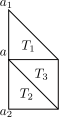
\includegraphics{../images/T1_Ch09-13}
\end{center}
\end{multicols}
On obtient alors 
\begin{equation}
    \frac{\partial}{\partial u_i^a} \int_{OA} \varpi x_2 \tilde{u}_1 \ud x_2 = - \psi_i^{a,T_1} - \psi_i^{a,T_2}
    \label{eq:Ch09-090}
\end{equation}
et finalement, la minimisation de $K$ donne 
\begin{equation}
    -\vec{f}^{a,T_1} - \cdots -\vec{f}^{a,T_n} + \vec{\varphi}^a + \vec{\psi}^a = 0 
    \label{eq:Ch09-091}
\end{equation}
On peut encore interpréter \eqref{eq:Ch09-091} comme exprimant l'équilibre du nœud a, à condition de rajouter aux forces appliquées
\begin{itemize}
    \item la force $\vec{\psi}^a = \vec{\psi}^{a,T_1}+ \vec{\psi}^{a,T_2}$ qui est la force concentrée équivalente en a aux forces de contact appliquées aux éléments entourant a. 
\end{itemize}

Ainsi, on peut interpréter la méthode des éléments finis comme exprimant l'équilibre des tous les nœuds sous l'action des forces élastiques exercées par chaque élément, et des forces extérieures (volumiques ou de contact) appliquées, ces forces étant rapportées aux nœuds. 
